\documentclass{article}
\usepackage[utf8]{inputenc}
\usepackage[spanish]{babel}
\usepackage{listings}
\usepackage{color}
\usepackage{verbatim}
\usepackage{float}
\usepackage{graphics,graphicx}
\usepackage[colorlinks]{hyperref}

\definecolor{dkgreen}{rgb}{0,0.6,0}
\definecolor{gray}{rgb}{0.5,0.5,0.5}
\definecolor{mauve}{rgb}{0.58,0,0.82}

\lstset{frame=tb,
  language=Java,
  aboveskip=3mm,
  belowskip=3mm,
  showstringspaces=false,
  columns=flexible,
  basicstyle={\small\ttfamily},
  numbers=none,
  numberstyle=\tiny\color{gray},
  keywordstyle=\color{blue},
  commentstyle=\color{dkgreen},
  stringstyle=\color{mauve},
  breaklines=true,
  breakatwhitespace=true,
  tabsize=3
}
\begin{document}
\begin{titlepage}
  \centering
  
\includegraphics[width=0.5\textwidth]{images/logo-ugr.png}\par
  \vspace{1cm}
  {\Large\scshape Gestión de Información en la Web \par}
  {\huge\bfseries Desarrollo de un Sistema de Recuperación de Información con la
  biblioteca \textit{Lucene} \par}
  \vspace{0.2cm}
  {\scshape Práctica 3 \par}
  \vfill
  {\large Víctor Vázquez Rodríguez  \par}
  {victorvazrod@correo.ugr.es \par}
  {76664636R}
  \vfill
  {\large Máster Universitario en Ingeniería Informática \par}
  \vspace{0.2cm}
  {Curso 2019/20 \par}
\end{titlepage}

\tableofcontents\newpage

\section{Introducción}

Hoy en día, el procesamiento de lenguaje natural (NLP por sus siglas en inglés)
es uno de los principales campos de estudio en inteligencia artificial y
\textit{deep learning}. Este campo se centra en la interpretación del lenguaje
humano por parte de ordenadores, permitiendo cosas como el control de
dispositivos con la voz o el análisis y traducción de textos.

Un aspecto muy importante a la hora de procesar y analizar lenguaje natural es
la representación que usamos del mismo, concretamente, cómo representamos las
palabras de forma que un ordenador pueda trabajar con ellas de forma eficiente y
obtener información relevante de su significado y su contexto. Desde el punto de
vista del \textit{machine learning}, podríamos interpretar las palabras de un
texto (o de cualquier conjunto de palabras) como valores de una variable
categórica, donde cada palabra distinta supone una categoría. Uno de los métodos
más comunes y usados para representar este tipo de variables es la codificación
\textit{one-hot}, que nos permite obtener un vector de valores númericos para
cada categoría.

No obstante, esta técnica presenta grandes limitaciones para el procesamiento de
lenguaje natural, de forma que surgen los \textit{word embeddings}. Se trata de
modelos apoyados en las redes neuronales para la proyección o incrustación
(traducción literal de \textit{embedding}) de palabras en un espacio
vectorial~\cite{definition}. En la sección \ref{sec:one-hot-limitations} de este
documento se explican las limitaciones de la codificación \textit{one-hot} y
por qué son necesarios los \textit{word embeddings}, mientras que en la sección
\ref{sec:techniques} se exponen algunas de las técnicas más utilizadas. Al
final, en la sección \ref{sec:example}, se muestra un ejemplo práctico de NLP
con \textit{word embeddings}.
\newpage
\section{Indexador}

Como su propio nombre indica, el indexador es la aplicación que construye el índice a partir de una colección de documentos dada. Se trata de una aplicación de línea de comandos que, como ya hemos indicado, hemos construido con \textbf{picocli}, una librería orientada a este tipo de aplicaciones. Esta librería nos permite definir \textit{flags} y otros parámetros de entrada para los comandos, facilitando su manejo. A continuación, se muestra la definición del comando creado para la indexación.

\begin{lstlisting}[language=Java]
@Command(name = "index", description = "Create or update an index from a set of documents.", mixinStandardHelpOptions = true, version = "index 1.0")
public class Index implements Callable<Integer> {

    @Parameters(paramLabel = "DIR", description = "Documents' directory to be indexed.", arity = "1..1")
    private File docsDir;

    @Option(names = { "-i", "--index" }, paramLabel = "INDEX", description = "Path to index. Defaults to /tmp/index.")
    private File indexFile = new File("/tmp/index");

    @Option(names = { "-s", "--stopwords" }, paramLabel = "STOPWORDS", description = "Stopwords file.", required = true)
    private File stopwordsFile;

    @Option(names = {"-u", "--update"}, description = "Update index instead of creating a new one.")
    private boolean update;

    public static void main(String... args) {
        int exitCode = new CommandLine(new Index()).execute(args);
        System.exit(exitCode);
    }
    
    @Override
    public Integer call() throws Exception {
        // Index documents
    }
}
\end{lstlisting}

Como se puede ver, nuestra aplicación requiere, por lo menos, de dos entradas: las rutas al fichero de palabras vacías (\textit{stopwords}) y a la colección de documentos. También se puede indicar una ruta para almacenar el índice aunque, si no se especifica, se usa \verb|/tmp/index| por defecto. Destacamos también el \textit{flag} \verb|-u|, el cuál permite indicar que se está actualizando un índice ya existente, con lo que no tenemos que realizar todo el proceso de nuevo si no es necesario.

En cuanto a la lógica que se encarga de realizar la indexación, es la siguiente:

\begin{lstlisting}[language=Java]
try {
    // Read stopwords from file
    var stopwords = readStopwords(stopwordsPath);

    // Set up index writer
    Directory dir = FSDirectory.open(indexPath);
    Analyzer analyzer = new SpanishAnalyzer(new CharArraySet(stopwords, true));
    IndexWriterConfig config = new IndexWriterConfig(analyzer);

    // Update index or create a new one
    if (update) {
        config.setOpenMode(OpenMode.CREATE_OR_APPEND);
    } else {
        config.setOpenMode(OpenMode.CREATE);
    }

    // Create index writer and process documents
    IndexWriter writer = new IndexWriter(dir, config);
    indexDocuments(writer, docsPath);

    // Close index writer
    writer.close();
} catch (Exception e) {
    System.out.println("Can't create index - Error: "+ e.getMessage());
    return 1;
}
\end{lstlisting}

El método \verb|indexDocuments| es el encargado de recorrer todos los archivos de la colección dada y llamar a \verb|indexDocument| para cada uno de ellos. Este último, extrae el texto del archivo PDF y añade el nuevo documento al índice, como se puede ver a continuación:

\begin{lstlisting}[language=Java]
public void indexDocument(IndexWriter writer, Path file) throws IOException {
    try (PDDocument pdf = PDDocument.load(file.toFile())) {
        // Extract text from PDF
        PDFTextStripper stripper = new PDFTextStripper();
        stripper.setLineSeparator("\n");
        stripper.setStartPage(1);
        String contents = stripper.getText(pdf);
        pdf.close();

        // Create Lucene document
        Document doc = new Document();

        // Add the path of the file
        doc.add(new StringField("path", file.toString(), Field.Store.YES));

        // Add the contents of the file
        doc.add(new TextField("contents", contents, Field.Store.NO));

        // Add the document to the index
        writer.addDocument(doc);
    }
}
\end{lstlisting}

Como se puede apreciar, indexamos tanto el contenido del documento como la ruta hacia el mismo.

\subsection{Manual de uso}

Usando el fichero \verb|jar| proporcionado, se puede ejecutar la aplicación de la siguiente manera:

\begin{lstlisting}
    java -jar indexer.jar --stopwords=[Ruta a fichero] --index=[Ruta a indice] [Ruta a coleccion]
\end{lstlisting}

Alternativamente, si se va a actualizar un índice ya creado, se puede usar:

\begin{lstlisting}
    java -jar indexer.jar -u --stopwords=[Ruta a fichero] --index=[Ruta a indice] [Ruta a coleccion]
\end{lstlisting}

\textbf{Nota:} Como ya se ha indicado anteriormente, no es completamente necesario indicar una ruta para el índice, usándose \verb|/tmp/index| por defecto.\newpage
\section{Buscador}

A diferencia del indexador, la aplicación del buscador sí que dispone de interfaz gráfica, permitiendo al usuario realizar múltiples consultas sobre el índice de manera sencilla en una misma sesión. Para construir esta interfaz, se ha usado \textbf{JavaFX}, obteniendo el resultado siguiente:

\begin{figure}[H]
    \centering
    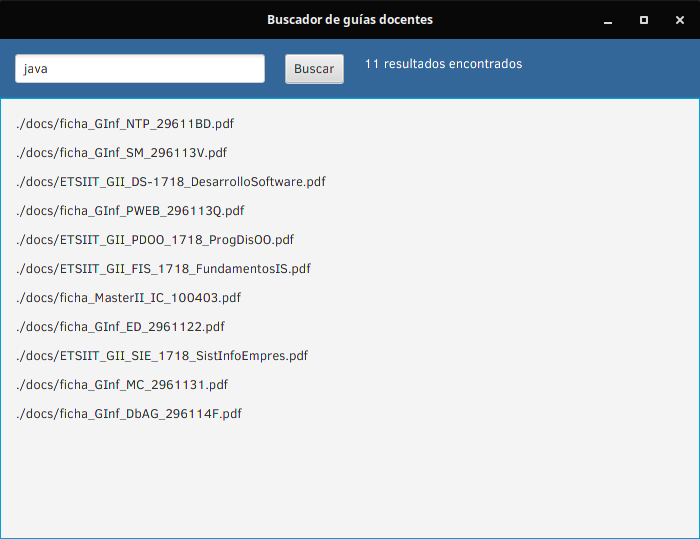
\includegraphics[width=1\linewidth]{images/searcher-ui.png}
\end{figure}

Para realizar las búsquedas, se necesitan tanto un \verb|QueryParser| para interpretar las consultas (con el mismo procedimiento usado para procesar los documentos) como un \verb|IndexSearcher| para realizar las búsquedas como tal sobre el índice. Estos objetos se construyen así:

\begin{lstlisting}[language=Java]
private IndexSearcher createIndexSearcher(Path indexPath) {
    IndexSearcher searcher = null;

    try {
        Directory indexDir = FSDirectory.open(indexPath);
        IndexReader reader = DirectoryReader.open(indexDir);
        searcher = new IndexSearcher(reader);
    } catch (IOException e) {
        System.out.println("Can't create index searcher - Error: " + e.getMessage());
        System.exit(1);
    }

    return searcher;
}

private QueryParser createQueryParser(Path stopwordsPath) {
    QueryParser parser = null;

    try {
        // Read stopwords from file
        var stopwords = readStopwords(stopwordsPath);

        // Create parser
        Analyzer analyzer = new SpanishAnalyzer(new CharArraySet(stopwords, true));
        parser = new QueryParser("contents", analyzer);
    } catch (IOException e) {
        System.out.println("Can't create query parser - Error: " + e.getMessage());
        System.exit(1);
    }

    return parser;
}
\end{lstlisting}

Una vez hecho esto, creamos la interfaz, dotando al botón de la funcionalidad de búsqueda, la cuál se puede ver a continuación:

\begin{lstlisting}
// Search button
Button searchBtn = new Button("Buscar");
searchBtn.setOnAction(new EventHandler<ActionEvent>() {

    @Override
    public void handle(ActionEvent e) {
        msgLabel.setText("");

        String inputString = queryTF.getText();
        if (inputString.isEmpty()) {
            msgLabel.setText("Por favor, introduce un termino para la busqueda");
            return;
        }

        try {
            Query query = parser.parse(inputString);
            var results = indexSearcher.search(query, 50).scoreDocs;
            resultsPane.refresh(results);
            msgLabel.setText(results.length +" resultados encontrados");
        } catch (ParseException pe) {
            msgLabel.setText("No se ha podido procesar la consulta");
        } catch (IOException ioe) {
            msgLabel.setText("Error en la consulta del indice");
        }
    }
});
\end{lstlisting}

Como su propio nombre indica, \verb|resultsPane| es el panel de la interfaz en el que se muestran los resultados. Llamando a su método \verb|refresh| con los nuevos resultados, lo que hacemos es refrescar el panel para mostrarlos. La construcción de los resultados en la interfaz se puede ver a continuación:

\begin{lstlisting}[language=Java]
public void refresh(ScoreDoc[] results) {
    this.getChildren().clear();

    for (int i = 0; i < results.length; i++) {
        try {
            Document doc = indexSearcher.doc(results[i].doc);
            this.getChildren().add(buildResult(doc));
        } catch (IOException e) {
            System.out.println("Can't retrieve result - Error: " + e.getMessage());
        }
    }
}

private HBox buildResult(Document doc) {
    HBox box = new HBox();
    box.setSpacing(15.0);

    // Add label with doc path
    Label pathLabel = new Label(doc.get("path"));
    box.getChildren().add(pathLabel);

    return box;
}
\end{lstlisting}

\subsection{Manual de uso}

Para lanzar la aplicación del buscador, debemos ejecutar el archivo \verb|jar| desde la línea de comandos, indicando las rutas al índice y al archivo de palabras vacías, de esta manera:

\begin{lstlisting}
java -jar searcher.jar --stopwords=[Ruta a fichero] --index=[Ruta a indice]
\end{lstlisting}

Una vez en la interfaz, para realizar una búsqueda sólo debe introducir los términos de la misma en el campo de texto y pulsar sobre el botón "Buscar".\newpage
\section{Referencias}

Para la realización de esta práctica se han usado algunas fuentes complementarias al guión proporcionado, las cuáles se indican a continuación:

\begin{itemize}
    \item \href{https://golang.org/doc/}{Documentación de Go}, usada para consultar dudas sobre ordenación de \textit{arrays}.
    \item \href{https://gin-gonic.com/docs/}{Documentación de Gin}, \textit{framework} usado para el desarrollo de la aplicación web.
    \item \href{https://gorm.io/docs/}{Documentación de GORM}, usada para consultar cómo se componían las consultas a la base de datos.
\end{itemize}\newpage
\end{document}
